\section{Task Definition}
\label{intro}

The task accomplished by this project is to build an AI agent for the game of Lunar Lander defined by openAI gym in Box2D format. Here, a lunar lander needs to land with zero velocity between the flags on a landing pad as shown in the figure. with a constant high reward. This is accomplished by Reinforcement Learning, particularly by applying different Deep Q-learning techniques. This project has explored Full DQN, Double DQN, and Dueling DQN, to solve the game. We have considered the game as solved when the agent starts getting an average reward of 200 over 100 consecutive episodes. Moreover, performances of different DQN variants are compared with baselines and oracle. \\

\begin{figure}[!ht]
%\begin{figure}%
%\vspace*{\fill}
\centering
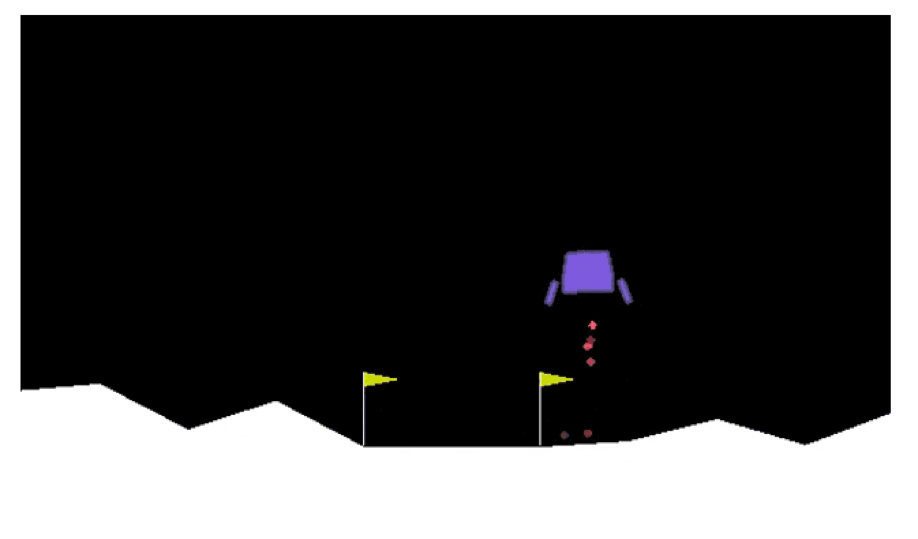
\includegraphics[scale=0.75,width=0.75\columnwidth]{figures/game.png}%
\caption{ Game Environment Screenshot}%
\label{fig:Visualization}%
\end{figure}
%\vfill}

Since this problem involves high dimensional and continuous state
space, standard Q-learning cannot solve this problem unless some amount of discretization is done. Due to above-mentioned difficulties, Deep Q-Network (DQN) was the choice. We plan to explore different variants of DQN (particularly DQN, Double DQN, and
Dueling network architecture).



